\section{Flat Combining}

Flat combining allows threads to cooperate when accessing a synchronized shared data structure to get greater overall throughput than even each of them operating serially. Careful engineering must be employed to implement a mechanism for cooperation that does not introduce the same synchronization issues as the original contended data structure. However, the same delegation mechanism can be reused in any data structure protected by a single global lock. 

\subsection{Physically-shared memory}

\begin{figure}[ht]
  \centering
  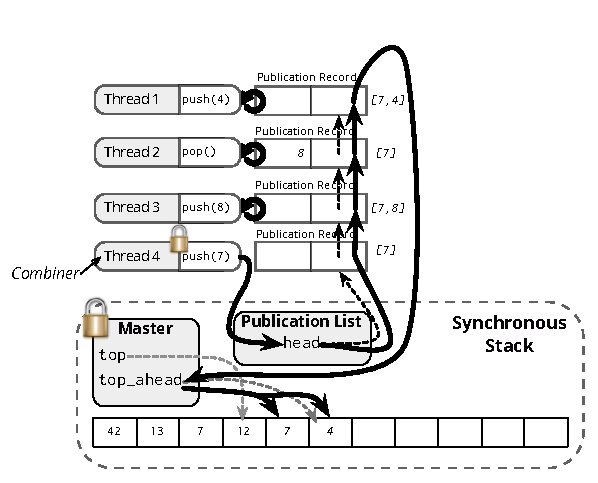
\includegraphics[width=0.5\textwidth]{figs/fc_shared_mem.pdf}
  \caption{Flat combining in shared memory. \TODO{walkthrough...}}
  \label{fig:fc_shared_mem}
\end{figure}

The benefits of flat-combining can be broken down into three components: improved locality, reduced synchronization, and data structure-specific optimization. Having a single thread bound to a particular core do a string of accesses trivially results in a lower cache miss rate than having multiple threads on multiple cores bring the data structure into cache each in turn.

The story for reducing synchronization is more complicated. The problem with having many threads attempt to acquire a lock is that as contention increases, there will be more failed synchronization attempts (failed \emph{compare and swap}, or \emph{CAS} operations), which must be retried until they succeed.
Instead of having most of the threads repeated fail on acquiring the lock, when threads observe that the lock has already been taken, they can delegate their work to the core with the lock by adding their requests to the structure's publication list. However, in a naive implementation, this operation still needs to perform synchronization every time a request is added to ensure inserts do not collide.
There is no way to avoid all synchronization, however, the cost may be amortized over many operations on the same data structure. Each thread must pay the synchronization cost to insert a publication record into the list once, but after that, it may reuse the record for subsequent accesses without synchronizing.

The final piece of the flat combining story is how operations are semantically combined using knowledge of how data structure accesses compose. All of the threads that did not acquire the lock block on their request until it is satisfied. Whichever thread did obtain the lock becomes the combiner. It iterates over the publication list, merging each non-empty publication record into a combined operation using a combining function defined by the data structure. When the pass is complete, the combined operation is applied to the actual data structure. The combiner thread then takes the aggregated results of the combined operation and distributes them to the correct requests in the publication list. When each request is fulfilled, the thread blocking on it wakes and continues, and finally the combiner thread releases the lock. If any publication requests remain, which could have come from threads that published their request after the combining thread had passed, one of them acquires the lock and becomes the new combiner.

\TODO{Add example of doing flat-combining on a global stack, discuss how pushes/pops are flattened.}

\subsection{In Grappa}

\begin{figure*}[t]
  \centering
  \begin{subfigure}[b]{0.43\textwidth}
    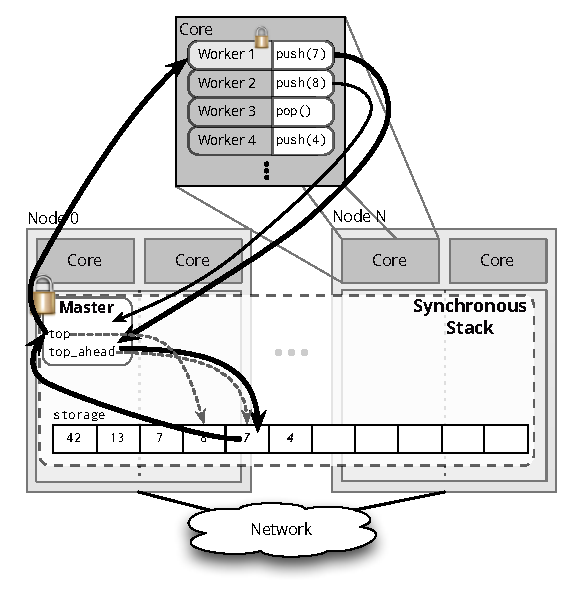
\includegraphics[width=\textwidth]{figs/stack_nofc.pdf}
    \caption{\emph{GlobalStack in Grappa.} Each access must synchronize with the head node (blocking if another worker is performing an operation), put or get its value in the stack's storage, release the lock on the master, and finally continue.}
    \label{fig:stacknofc}
  \end{subfigure}%
  \hspace{0.05\textwidth}
  \begin{subfigure}[b]{0.43\textwidth}
    \centering
    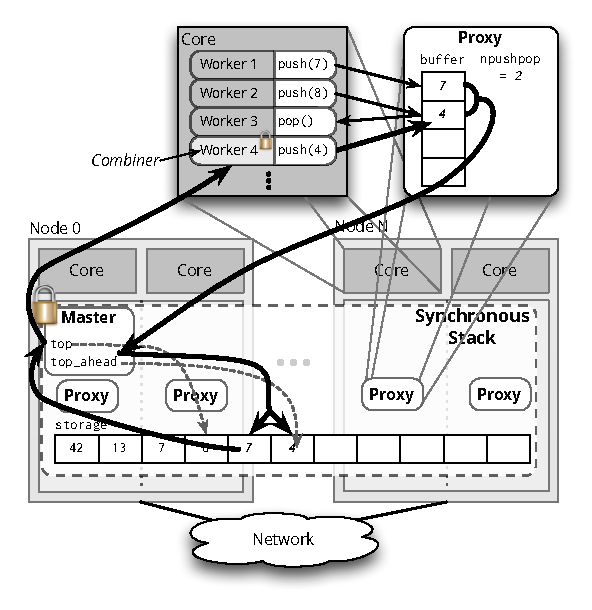
\includegraphics[width=\textwidth]{figs/stack_fc.pdf}
    \caption{\emph{GlobalStack in Grappa.} Each access must synchronize with the head node (blocking if another worker is performing an operation), put or get its value in the stack's storage, release the lock on the master, and finally continue.}
    \label{fig:stackfc}
  \end{subfigure}
  \caption{\emph{GlobalStack in Grappa.}}
  \label{fig:stack}
\end{figure*}

The cost of performing synchronization remotely on a distributed data structure motivates applying the flat-combining paradigm to Grappa data structures. Instead of all of the workers on a core sending messages to do remote synchronization independently, flat-combining can allow all of the workers to share a single remote synchronization operation. In a way, the Grappa runtime is already reducing synchronization traffic when it aggregates small messages that are all going to the same destination. However, it doesn't know what the operations are doing, so it must still serialize, pack, transmit, perform the operation on the remote side, and send a response for each message. Flat combining is about ``teaching'' it how to more efficiently perform many operations remotely in certain special cases.

In a PGAS setting, and in Grappa in particular, a number of different choices are made when implementing flat combining. Because memory is physically distributed, locality must be made explicit. In addition, in Grappa there are orders of magnitude more concurrent threads (``workers'') accessing shared data structures. Typically around a thousand are needed per core to tolerate the latency of remote operations, so in a cluster of machines, there are easily millions of workers. Therefore, a different scheme for managing many threads is necessary.

Flat-combined global data structures have a local publication list on each core which serve as proxies to the global structure and are used to combine requests. Workers add their requests to the local publication list by issuing operations on their local proxy and then block waiting for their requests to be satisfied. Similar to the shared-memory case, one requesting worker is chosen to combine requests and perform the combined operation globally. This worker walks the local publication list, combining requests into a local request object as it goes. If it is possible to service a request locally, as it is on some data structures such as matching pushes and pops to a stack, the combiner can satisfy the requests and wake the correct workers even before synchronizing globally. The combiner then issues the combined data structure operation globally. In most cases, this means communicating with whichever core holds the ``lock-protected'' field that maintains sequential consistency. In the case of a global stack, this is the ``master'' \emph{top} pointer which must be incremented on pushes and decremented on pops. On the core where global synchronization is occurring, there must be synchronization between the multiple synchronization requests arriving from other cores.

At this point we have traded off one remote synchronization per operation for an additional local synchronization per operation and some number fewer remote synchronizations (depending on the amount of combining that occurs). This would likely result in a net benefit due to local synchronization being inherently cheaper. However, because of the way the Grappa runtime schedules computation, it is actually possible to get the correct mutual exclusion/atomicity without any additional synchronization overhead.

By design, each core in Grappa operates independently of the other cores. Workers are scheduled cooperatively, so each worker can assume atomicity until it performs an operation that yields to the scheduler, such as a remote call. Therefore workers within a core can cooperate without any explicit synchronization operations requiring memory fences. This allows them to publish requests to the local  proxy very inexpensively, eliminating the need for a complex synchronization-amortizing queue. This has the added benefit that there will be no unused publication records, which could have become a problem with thousands of workers. Further, remote operations are processed through the same cooperative-multithreading scheduler on the remote side, so combined operations are trivially serialized and atomic.

\paragraph{Correctness}
\TODO{(are these arguments correct??)}

It may not be immediately obvious why this two-level version of flat combining preserves sequential consistency. The combining operations that are performed locally among requests on a single core must preserve the illusion of sequential order; this is unchanged from shared-memory flat-combining. When combined operations are applied globally, they are serialized at the ``master'' core for a given synchronization context. The global order is essentially the concatenation of each core's serialized updates. In the case where operations are satisfied locally (by matching up with other local operations), by definition these must be independent of other operations, so they can conceptually be placed anywhere in the global ordering (or even ignored completely in the global ordering).

In the spirit of the Data-Race-Free-0 Model (guaranteeing sequential consistency for data-race free programs), operations on the global data structure are considered to be made atomic by a conceptual global ``lock'' on the data structure. Atomicity and freedom from data races in the case of multiple data structures and other synchronization must be guaranteed externally, just as in any multithreaded shared-memory program.

\section{FC Framework}
In order to leverage the flat-combining paradigm in Grappa, we implemented a generic flat-combining framework which can be used to improve performance for a number of global data structures. The FC framework handles the common problems of managing the combiners, handling worker wake-ups, and maintaining progress. When hooking into the framework, each data structure implementation need only define how to combine operations and globally commit them.

The Grappa FC framework takes a different approach than the original flat-combining work for expressing how operations combine. In the original work, an explicit publication list is built up, and when the combiner scans over the list, it has a structure that it uses to accumulate requests in a logical way. In the case of the stack, for instance, it is a thread-local stack, which it can use to immediately match up pushes and pops. In the Grappa implementation, each worker's actions are atomic anyway, so rather than creating an explicit request list, the combiner object (or \emph{proxy}) is instantiated ahead of time for the data structure, and each worker does its own local combining into that structure before blocking. This reduces the space blowout of a large dynamically-sized publication list (with associated caching issues), and does not overly affect the expression of combining.

Using this style, each global data structure must define the following:
\begin{enumerate}
  \item A local \emph{proxy} data structure for doing combining.
  \item \emph{Combining methods} that operate on the local proxy.
  \item A \emph{sync} method that globally commits the proxy's state.
\end{enumerate}

Being conservative about SC, workers typically block when issuing these requests, so the framework must also take care of delivering results and waking the correct workers. The flat-combining framework is responsible for ensuring that all of the combined operations eventually get committed. There are a number of ways progress could be guaranteed, but one of the simplest is to take an approach in the spirit of the original flat-combining, which is to ensure that as long as there are any outstanding requests, there is at least one worker committing a combined operation. When that combined operation finishes, if there are still outstanding requests that have built up in the meantime, another blocked worker is chosen to do another combined synchronization.

One could imagine other synchronization policies that would ensure progress but allow more combining to occur before synchronizing. For instance, local combining could continue until all workers are blocked. However, this would require the flat-combining framework to track the activity of the workers on a core, and additionally would add latency unless the system saved enough active workers to tolerate the latency of the global commit action. As it is, the one-in-flight policy implemented performs well, and does not require any coupling with the Grappa scheduler. Exploration of other policies is left for future work.

The flat combining framework transparently wraps the \emph{proxy} object. Behind this layer of indirection, it manages multiple copies of the proxy so that, as discussed above, there is always at least one being committed and one to receive additional combining operations.

% explain simple non-combined global data structures in Grappa section...

\subsection{Global Stack}
To demonstrate the flat-combining framework, we revisit the Global Stack example from earlier. Recall that the ``master'' core owns the \texttt{top} index, which indicates where the top of the stack currently is in the stack's allocated global storage. In the non-combining case, each call to \texttt{push} must do an atomic increment of \texttt{top} to claim storage, then write to that location, then finally return. 



